\documentclass[12pt]{article}
\setlength{\oddsidemargin}{0in}
\setlength{\evensidemargin}{0in}
\setlength{\textwidth}{6.5in}
\setlength{\parindent}{0in}
\setlength{\parskip}{\baselineskip}

\usepackage{xcolor}
\usepackage{amsmath,amsfonts,amssymb}
\usepackage{qtree}
\usepackage{enumerate}
\usepackage{multirow}
\usepackage{graphicx}
\usepackage{forest}
\usepackage{colortbl}

\begin{document}

CSCI 4448 Spring 2016 \hfill Project Write-up 6\\
Ethan Wright \\
Julio Lemos \\
Nhan Nguyen \\

\hrulefill
%%%%%%%%%%%%%%%%%%%%%%%%% SECTION 1  %%%%%%%%%%%%%%%%%%%%%%%%%
\begin{enumerate}
  \item \textbf{Features Implemented} 
    \vspace{1cm}
    \\     
    \begin{tabular}{| l | l | } 
      \hline
      \textbf{ID} & \textbf{Feature}  \\ \hline
      BR-003 & Replication factor of 3 for data consistency \\ \hline
      UR-001 & User can search ingredients by category \\ \hline
      UR-002 & User can search ingredients by query \\ \hline
      UR-003 & User can enter dietary restrictions \\ \hline
      UR-004 & User can enter an optimal price range \\ \hline
      UR-005 & User can save a dietary preference/restriction \\ \hline
      UR-007 & User can generate recipe list at any point \\ \hline
      UR-008 & User can remove an ingredient from their list \\ \hline
      NFR-002 & Return at least 3 hits in under one second \\ \hline
      NFR-004 & Database results cached locally \\ \hline
      NFR-005 & Set partition size for Database \\ \hline
    \end{tabular}

  \newpage
  \item \textbf{Features Not Implemented}
    \vspace{1cm}
    \\
    \begin{tabular}{| l | l |}
      \hline
      \textbf{ID} & \textbf{Feature} \\ \hline
      BR-001 & Ingredients must be able to include sponsor links \\ \hline
      BR-002 & Collect user data for later processing \\ \hline
      UR-006 & User can select importance value of dietary restriction \\ \hline
      NFR-001 & Show 10 recipes upon search \\ \hline
      NFR-003 & Less than one second load time for initial website \\ \hline
    \end{tabular} \\

  \newpage
  \begin{figure}
      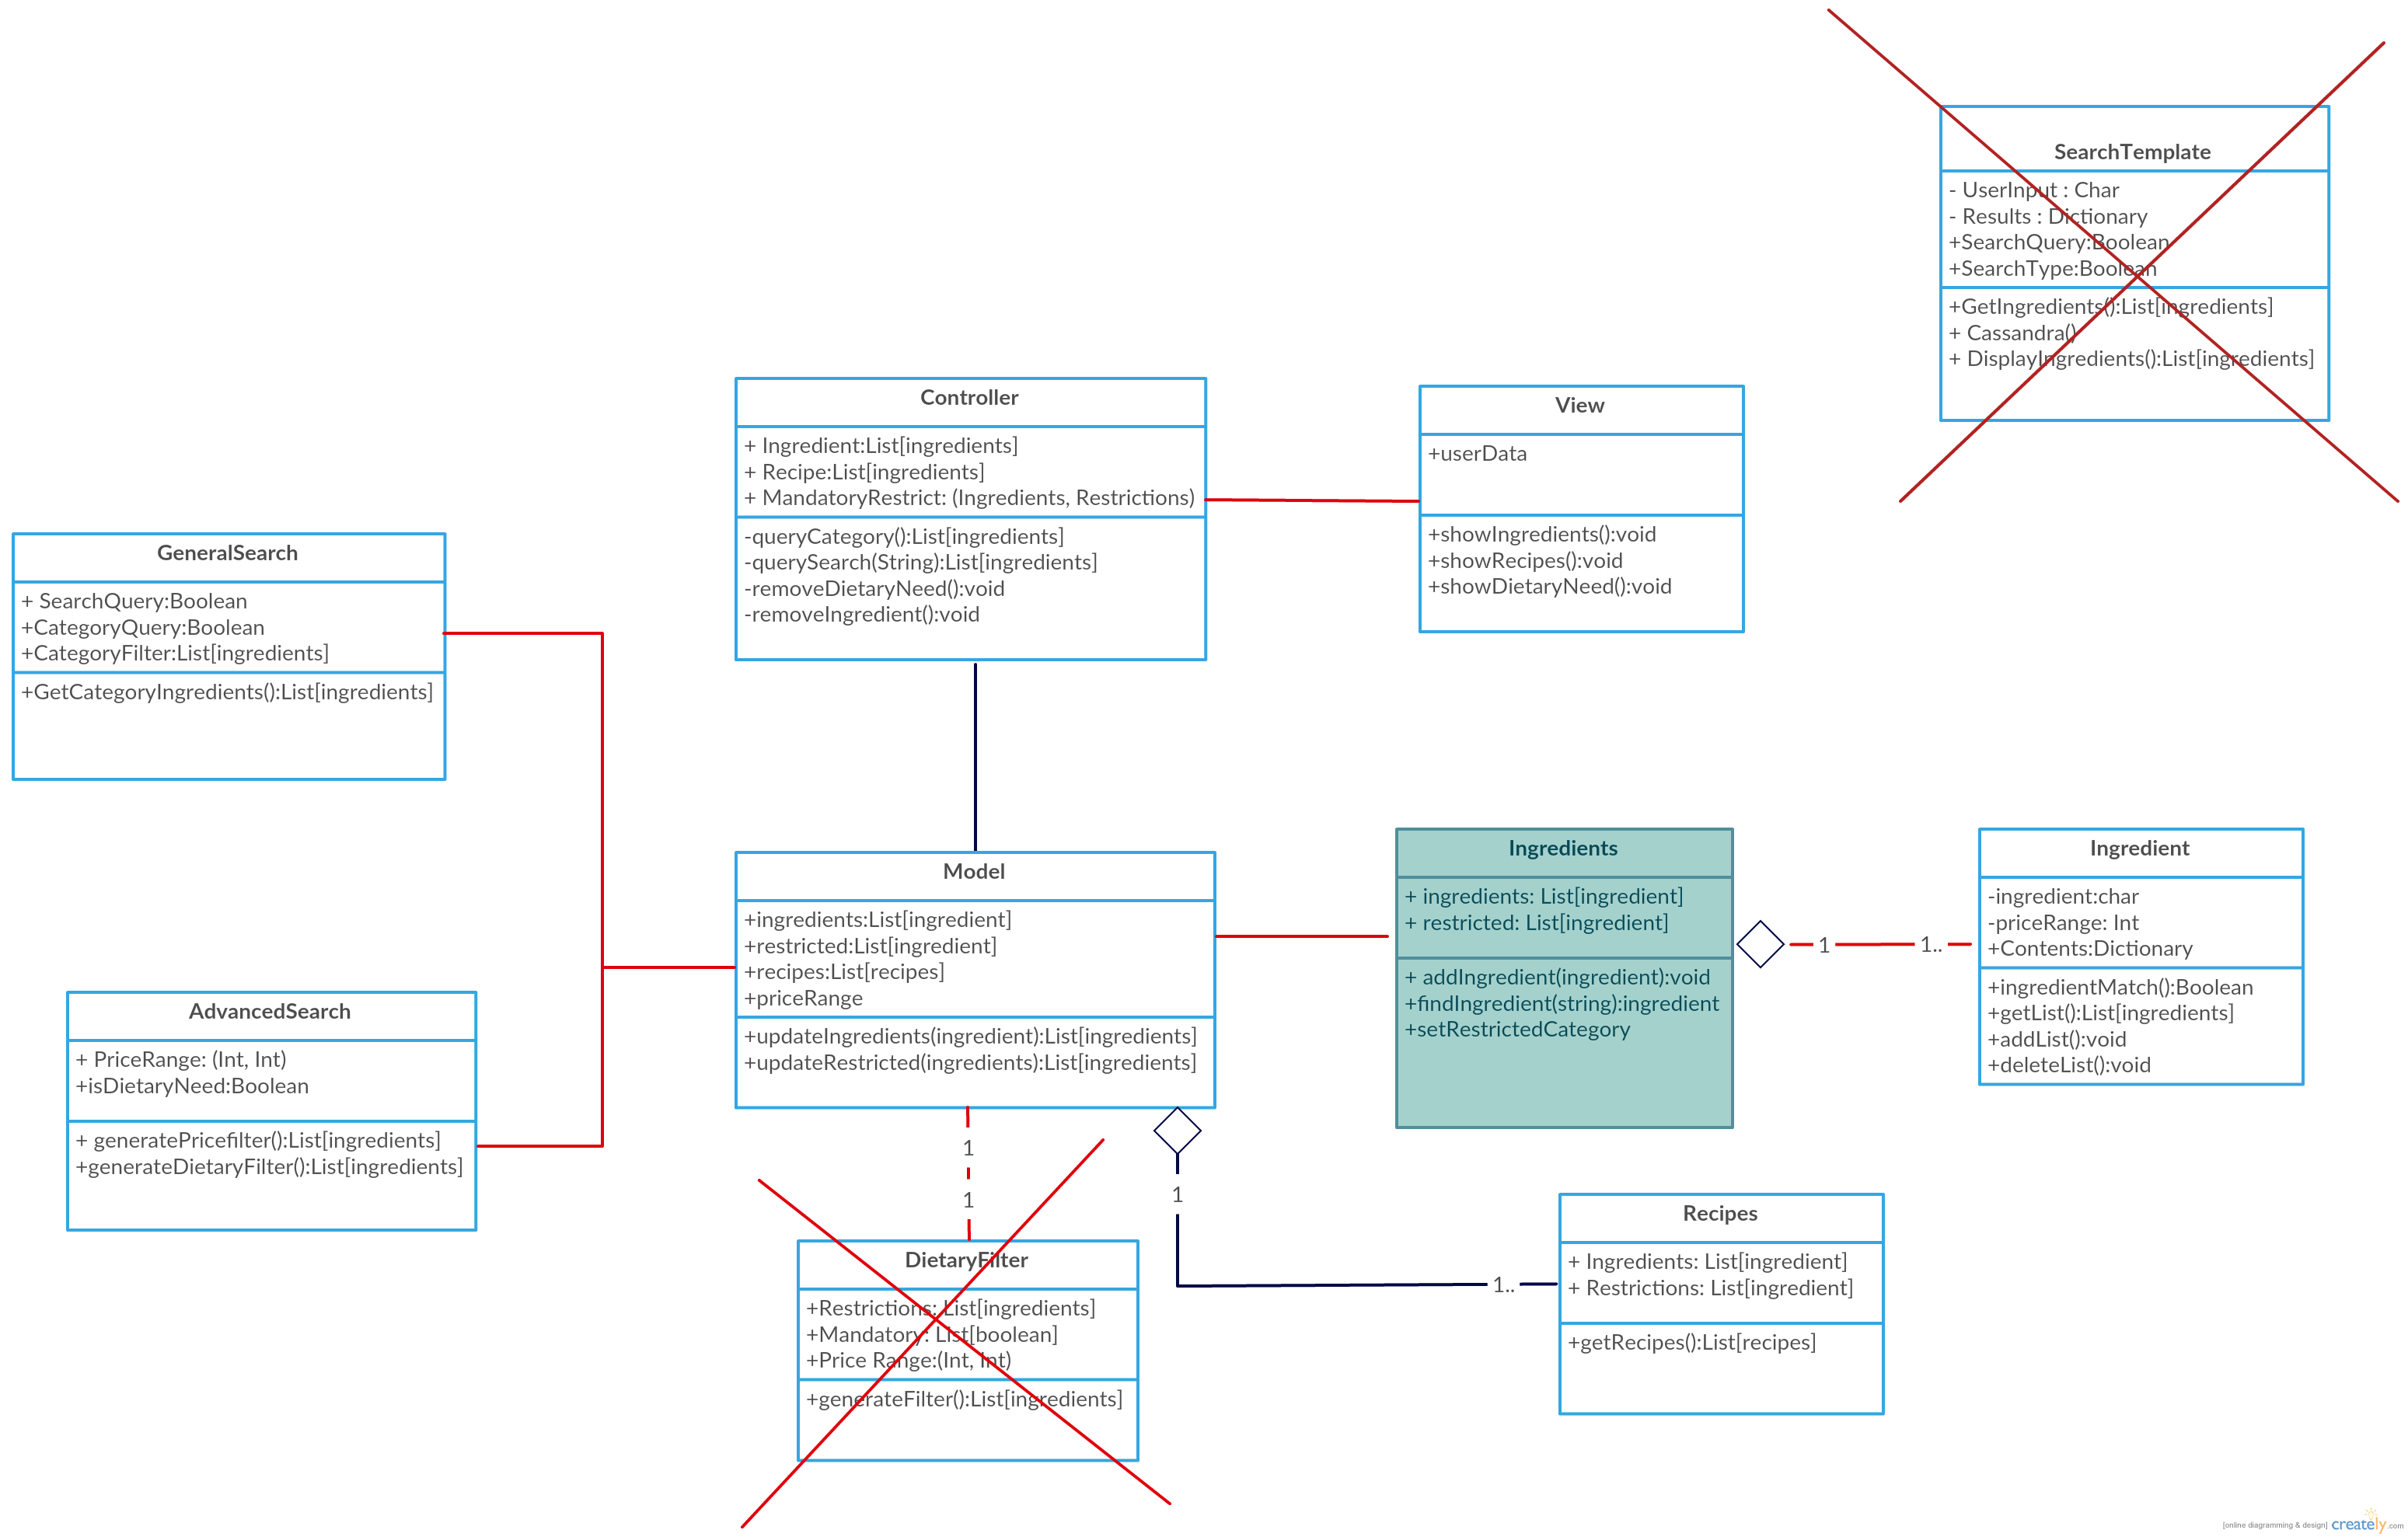
\includegraphics[width=\linewidth]{newclass.png}
      \caption{New Class Diagram}
      \label{fig: newclass}
  \end{figure}


  \begin{figure}
    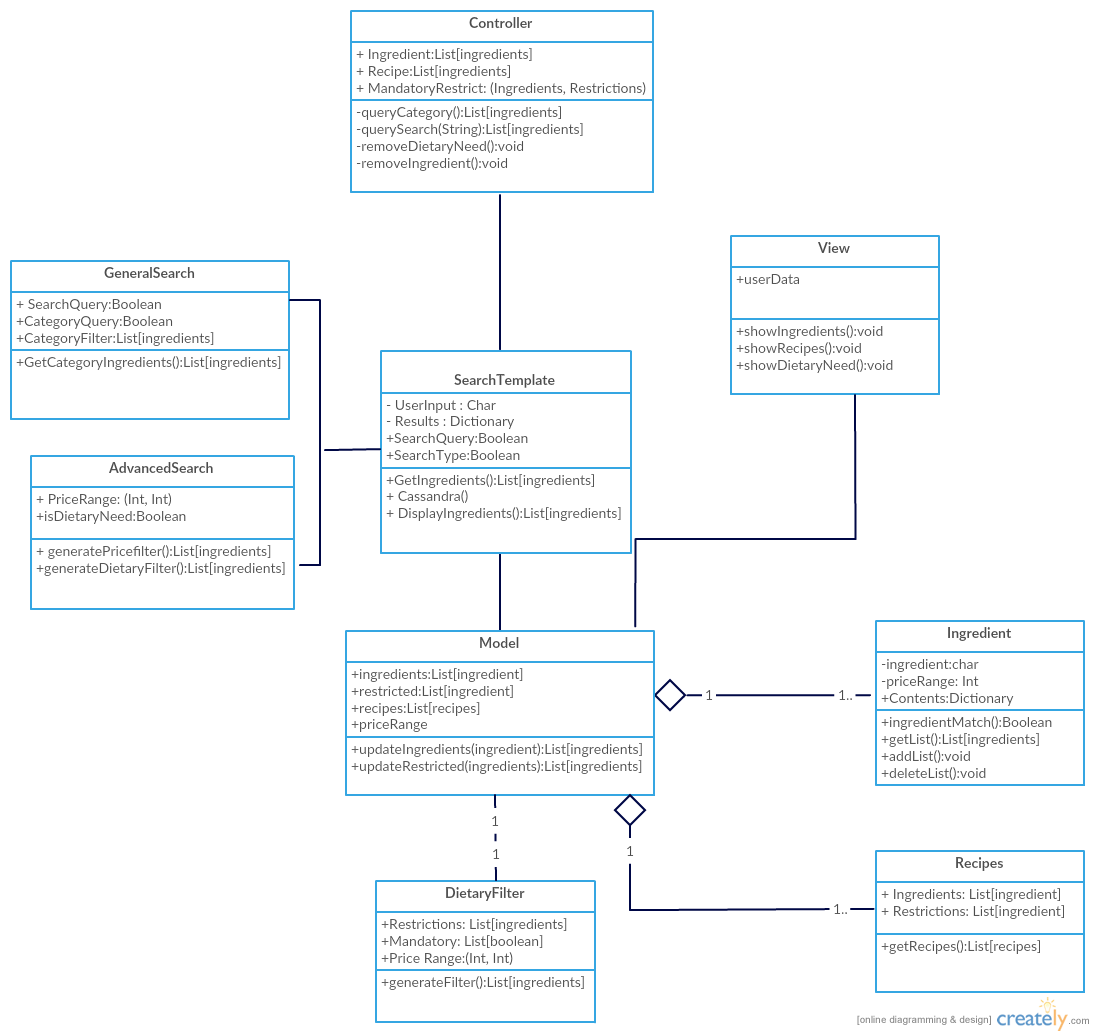
\includegraphics[width=\linewidth]{oldclass.png}
    \caption{Old Class Diagram}
    \label{fig: oldclass}
  \end{figure}

  \newpage
  \item \textbf{Design Patterns Used}
    \begin{enumerate}[i.]
      \item \textit{Mode View Controller} \\
        For this design pattern we attempted to implement a class structure that followed a similar pattern.
        We didn't use the actual Spring MVC that we worked on in class, but instead tried to implement 
        our own version of it in the Class Diagram as well as in the actual implementation of our program.
      \item \textit{Chain of Command} \\ 
        The chain of command pattern was much more difficult to actually implement in our software. Our initial
        class diagram implemented it fairly well (after we added it during refactoring) but we found that this
        was the most difficult to implement once we actually started designing. This was because once we started 
        having to make changes to our design while coding it was hard to accurately maintain the chain of command
        without stepping back and remapping our core design. As a software developer, it's certainly hard to 
        take some time when coding to plan things out. As they say, days of coding save you hours of design. 
        This was certainly the case for the implementation of chain of command.
      \item \textit{Template} \\
        Template proved to be highly beneficial for us during this project. We used template initially to 
        split up our search into multiple levels, but then we used similar structures to help us implement our MVC.
        With our model class we were able to create set parameters for the user and the database that we could then
        extend to the given classes such as ingredients and recipe, and it was incredibly usefull to have the template
        design pattern in the back of our head when doing this construction.
    \end{enumerate}
  \newpage
  \item \textbf{What we learned about process of analysis and design after implementing a system} 
    \vspace{1cm}
    \\
    The biggest take away about the process of analysis and design is the fact that it has to be an ongoing process.
    While we greatly enjoyed the aspects of the class that focused on the architecture of the project, we found that
    once we got to coding things started to shift that we weren't able to account for. Had we been using an agile
    approach that appropriatley accomodated for creating design patterns every day that we were going to do a 
    programming sprint we likely would have been more sucessful. Instead we would spend a week or two doing our
    design and reworking it, and then we would dive into the programming agnostic to any change in design and powering
    through. This waterfall method of software development certainly hindered our prospect of sucess because we
    weren't able to shift our patterns and architecture of the project as we went.
   \end{enumerate}
\end{document}
















